% =============================================================================
% Guía personal de exposición — Rol C (puntos 3 y 4), 3 minutos
% Uso interno de preparación; no forma parte del informe.
% Las diapositivas están en dashboard/index.html, vista "Rol C: Tendencias y Fourier".
% Compilar desde documentos/presentacion/:  pdflatex guion_exposicion_rol_c.tex
% =============================================================================
\documentclass[11pt,letterpaper]{article}
\usepackage[utf8]{inputenc}
\usepackage[T1]{fontenc}
\usepackage[spanish,es-nodecimaldot,es-noshorthands]{babel}
\usepackage{lmodern}
\usepackage[margin=2.2cm]{geometry}
\usepackage{amsmath}
\usepackage{graphicx}
\usepackage{booktabs}
\usepackage{tabularx}
\usepackage{float}
\usepackage{caption}
\usepackage{xcolor}
\usepackage{tcolorbox}
\usepackage{enumitem}
\usepackage[hidelinks]{hyperref}
\graphicspath{{../../figuras/}}
\captionsetup{font=small,labelfont=bf}
\setlist{itemsep=2pt,topsep=3pt}

\definecolor{guion}{HTML}{1F5F6B}
\newtcolorbox{guion}{colback=guion!6,colframe=guion,boxrule=0.6pt,arc=2pt,
  left=6pt,right=6pt,top=4pt,bottom=4pt,title=Qué decir,fonttitle=\bfseries\small}
\newtcolorbox{cifras}{colback=orange!6,colframe=orange!70!black,boxrule=0.6pt,arc=2pt,
  left=6pt,right=6pt,top=4pt,bottom=4pt,title=Cifras que debes recordar,fonttitle=\bfseries\small}

\title{Guía de exposición del Rol C\\\large Tendencias (punto 3) y Fourier (punto 4) en 3 minutos}
\author{Preparación personal --- Tomás Gómez}
\date{}

\begin{document}
\sloppy
\maketitle

\section*{Idea central}

Si solo pudieras decir una frase, sería esta:
\begin{quote}
\emph{``Desde 2010 llueve menos en invierno, por eso se acumula menos nieve y el río lleva menos agua todo el
año. La cuenca almacena y retrasa la lluvia, y por eso la sequía se nota más y dura más en el caudal que en la
precipitación.''}
\end{quote}
Todo lo demás de la exposición son las pruebas de esa frase. Al profesor le importa que expliques la
\textbf{física} (la interpretación vale el 25\,\% de la nota oral) y que defiendas las \textbf{decisiones de
método} (10\,\%), no que leas cifras. Usa las cifras como evidencia, no como contenido.

\section*{Mapa de los 3 minutos}

\begin{table}[H]
\centering\small
\begin{tabularx}{\textwidth}{c l c X}
\toprule
\# & Pregunta que respondes & Tiempo & Mensaje en una frase \\
\midrule
01 & ¿Qué cambia, cuánto y en qué meses? (3.3--3.5) & 40 s & El caudal baja en los 12 meses; la lluvia solo en invierno. \\
02 & ¿Lineal o salto? ¿Robusto? (3.4--3.5) & 35 s & El cambio se concentra después de 2007--2010; no se distingue tendencia de salto. \\
03 & ¿A qué se debe? (3.6) & 45 s & El caudal cae en proporción a la lluvia (elasticidad $\approx$1.1); hay un pequeño déficit extra. \\
04 & ¿En qué escalas varía? (4.2) & 40 s & La cuenca filtra la lluvia: entra ruido casi blanco y sale una señal roja; solo el ciclo anual es un pico robusto. \\
05 & Síntesis & 20 s & Menos lluvia invernal, menos nieve, menos río, todo el año. \\
\midrule
 & \textbf{Total} & \textbf{3:00} & Unas 420 palabras a ritmo normal (140 por minuto). \\
\bottomrule
\end{tabularx}
\end{table}

Ensaya con cronómetro. Si vas atrasado, recorta la diapositiva 02 (di solo la primera frase) y nunca la 03 ni
la 04, que responden directamente a las preguntas 3.6 y 4.2.

% -----------------------------------------------------------------------------
\section{Diapositiva 01 --- ¿Qué cambia? (40 s)}

\begin{figure}[H]
\centering
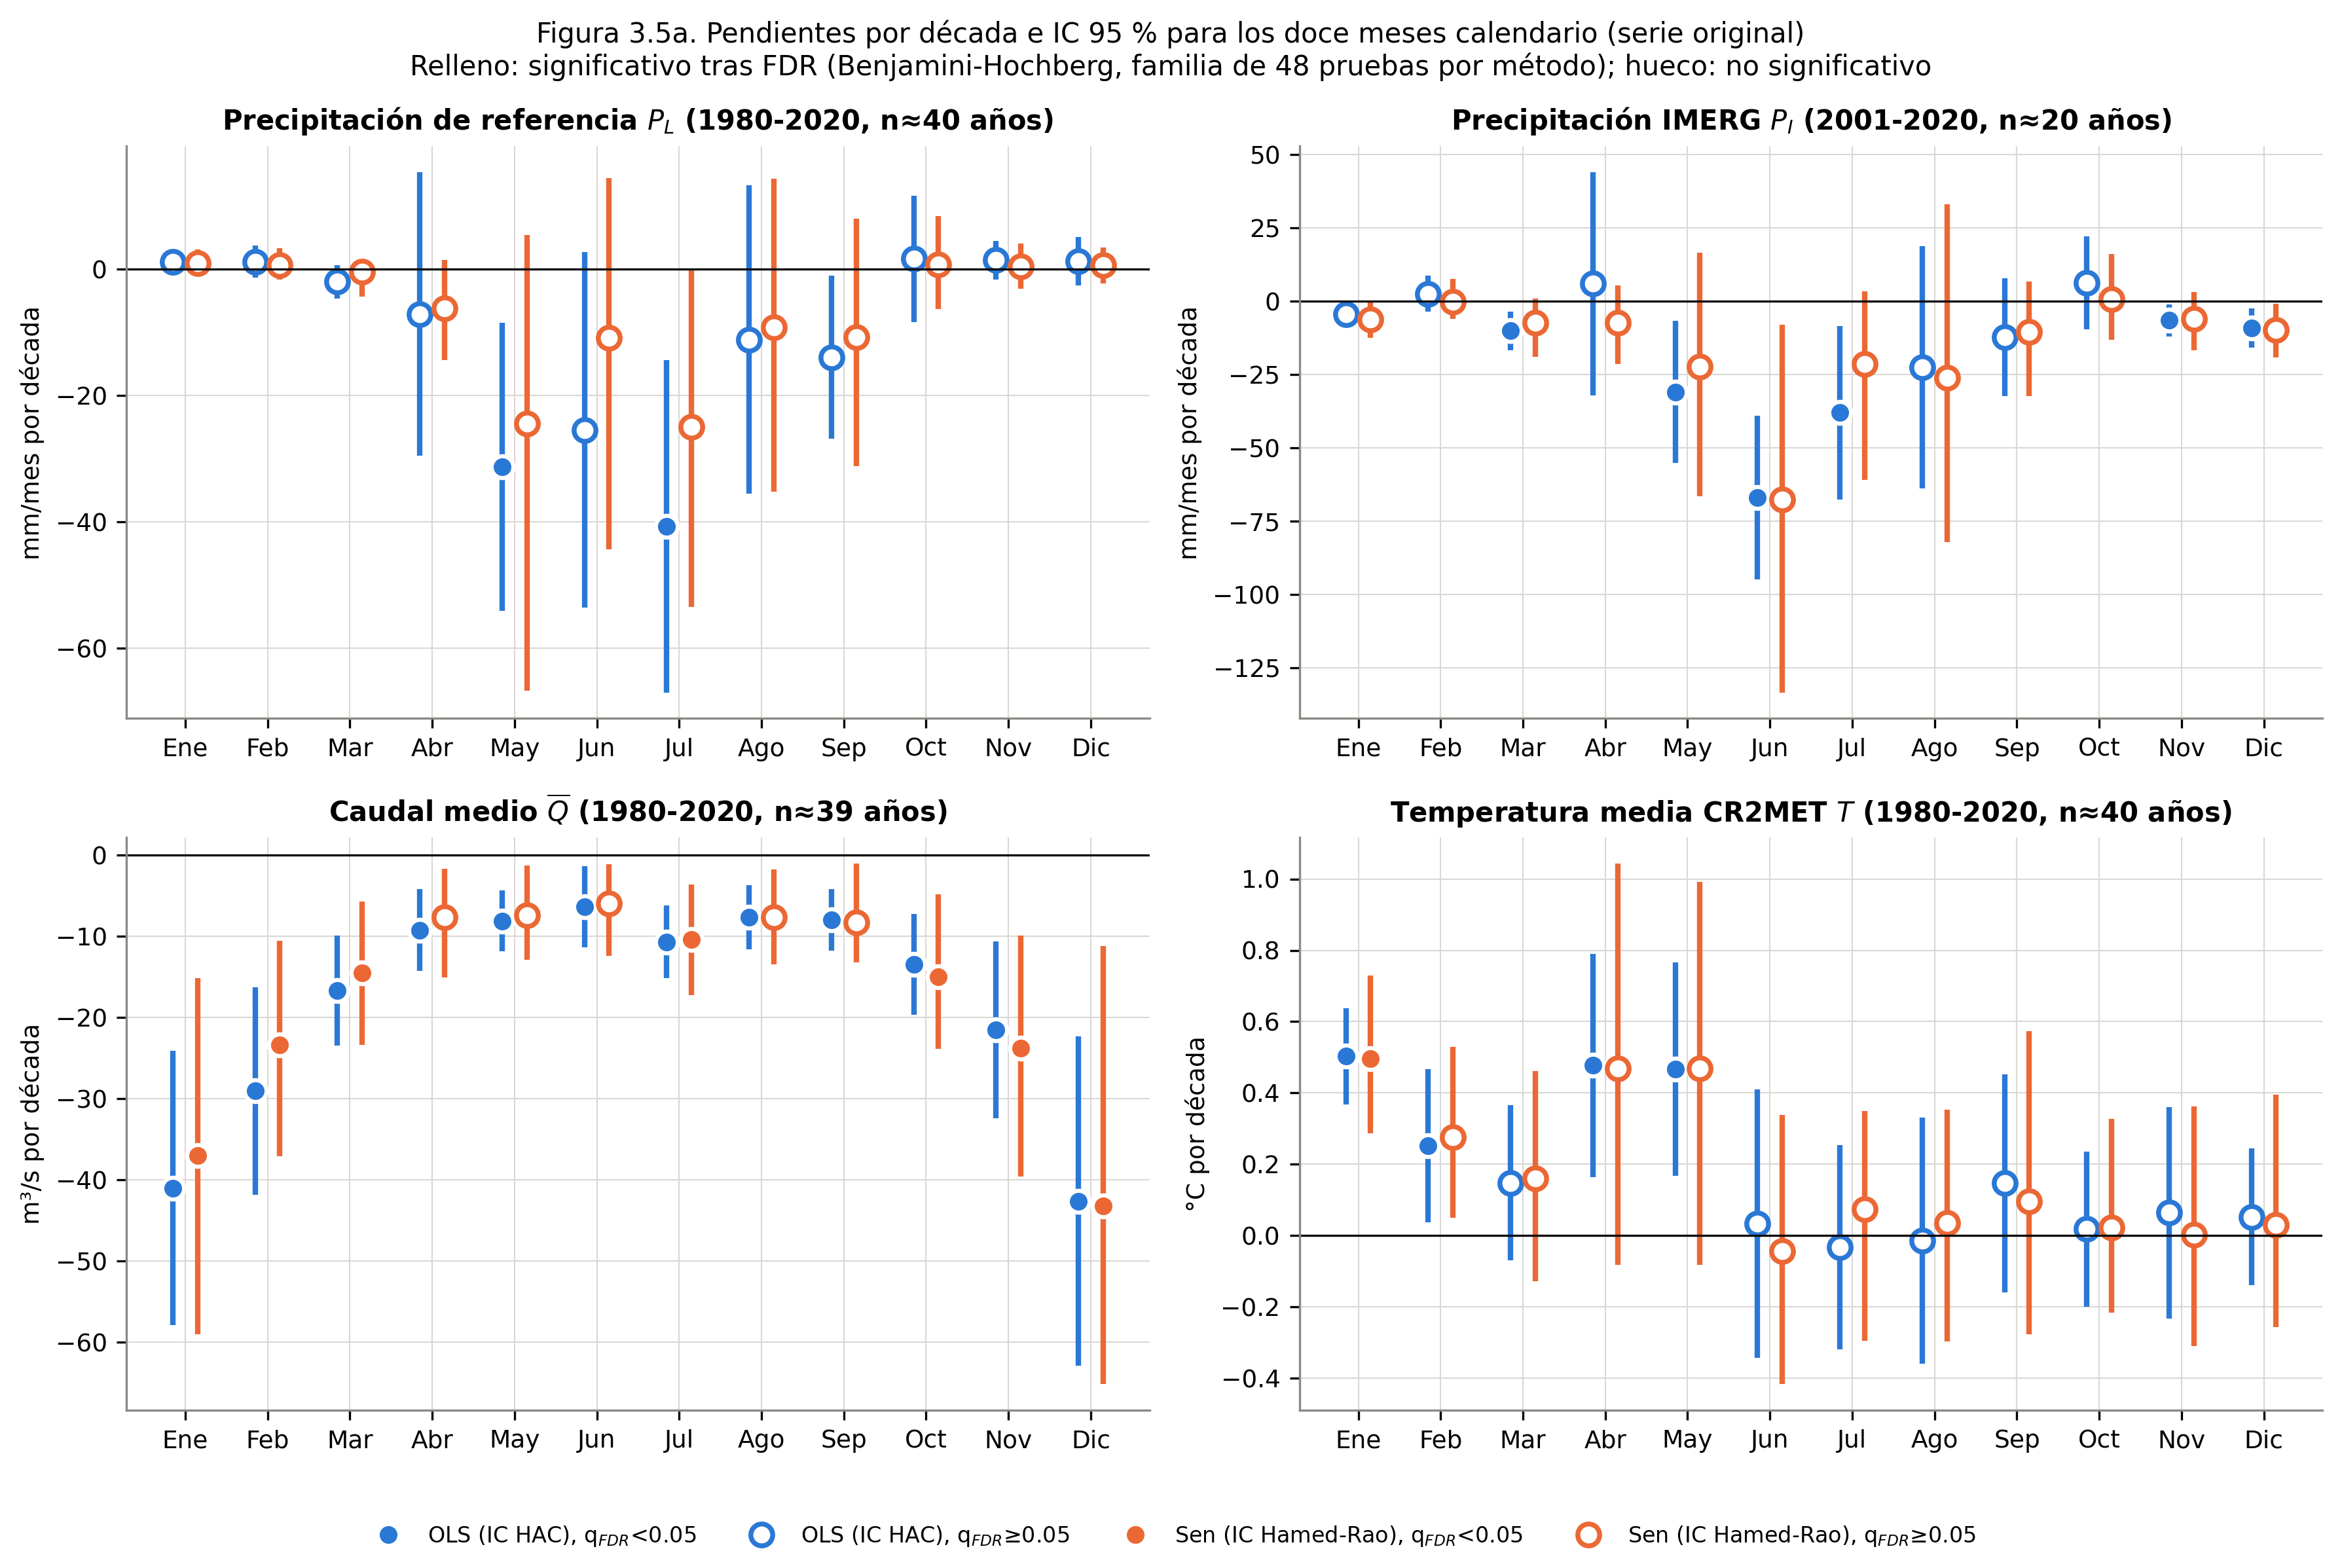
\includegraphics[width=0.9\textwidth]{figura_3_5a_pendientes_mensuales_ic.png}
\caption{Versión del informe de la diapositiva 01 (figura 3.5a). En el dashboard se muestran P$_L$ y Q en
\% de la media mensual por década para ponerlas en una escala común.}
\end{figure}

\paragraph{Cómo se lee la gráfica.} Cada punto es la pendiente OLS de un mes calendario a lo largo de los
40 años (por ejemplo, todos los eneros de 1980 a 2020). La barra vertical es el intervalo de confianza del
95\,\% con errores HAC. El punto \textbf{relleno} es significativo después de corregir por comparaciones
múltiples (FDR); el \textbf{hueco} no lo es. Un punto bajo cero indica que ese mes se está secando.

\paragraph{Lo fundamental.} El patrón estacional. La lluvia solo cae en mayo--julio, que es cuando se acumula
la nieve; en verano no cambia. El caudal cae en \emph{todos} los meses, y más en diciembre--enero, que es el
deshielo. Que la lluvia cambie en invierno y el río en verano es la huella del almacenamiento nival.

\begin{guion}
``Evaluamos la tendencia de cada mes calendario por separado. La precipitación disminuye solo en los meses de
invierno, mayo y julio, entre un 24 y un 28\,\% de su media por década. En cambio, el caudal disminuye en los
doce meses, alrededor de 18 metros cúbicos por segundo por década, y su caída más grande ocurre en
diciembre y enero, en pleno deshielo. Es decir, el déficit de lluvia invernal reaparece en el río meses
después. La temperatura de ERA5-Land sube unas tres décimas de grado por década, pero en veinte años eso no
es significativo.''
\end{guion}

\begin{cifras}
\begin{itemize}
\item Q: $-18.2$~m$^3$/s por década (IC $[-26.7,\,-9.7]$, $p<0.001$); los 12 meses son significativos tras FDR.
\item P$_L$: $-10.2$~mm/mes por década ($p=0.004$), concentrada en mayo--julio; solo mayo y julio superan el FDR.
\item IMERG: $-15.5$~mm/mes por década (2000--2020). T: $+0.28$~$^\circ$C por década ($p=0.27$, no significativo).
\end{itemize}
\end{cifras}

\paragraph{Si te preguntan\ldots}
\begin{itemize}
\item \emph{¿Por qué errores HAC?} Porque los residuos están autocorrelacionados (en el caudal, el rezago 1
es 0.78) y los errores usuales subestimarían la incertidumbre.
\item \emph{¿Por qué FDR?} Hicimos 48 pruebas (12 meses por 4 variables). Al 5\,\%, unas 2 o 3 saldrían
significativas solo por azar.
\item \emph{¿Por qué no muestras también anomalías y anomalías estandarizadas?} Dentro de un mismo mes, restar
la media o dividir por la desviación no cambia la prueba; lo verificamos numéricamente. No son evidencia
independiente.
\end{itemize}

% -----------------------------------------------------------------------------
\section{Diapositiva 02 --- ¿Tendencia o salto? (35 s)}

\begin{figure}[H]
\centering
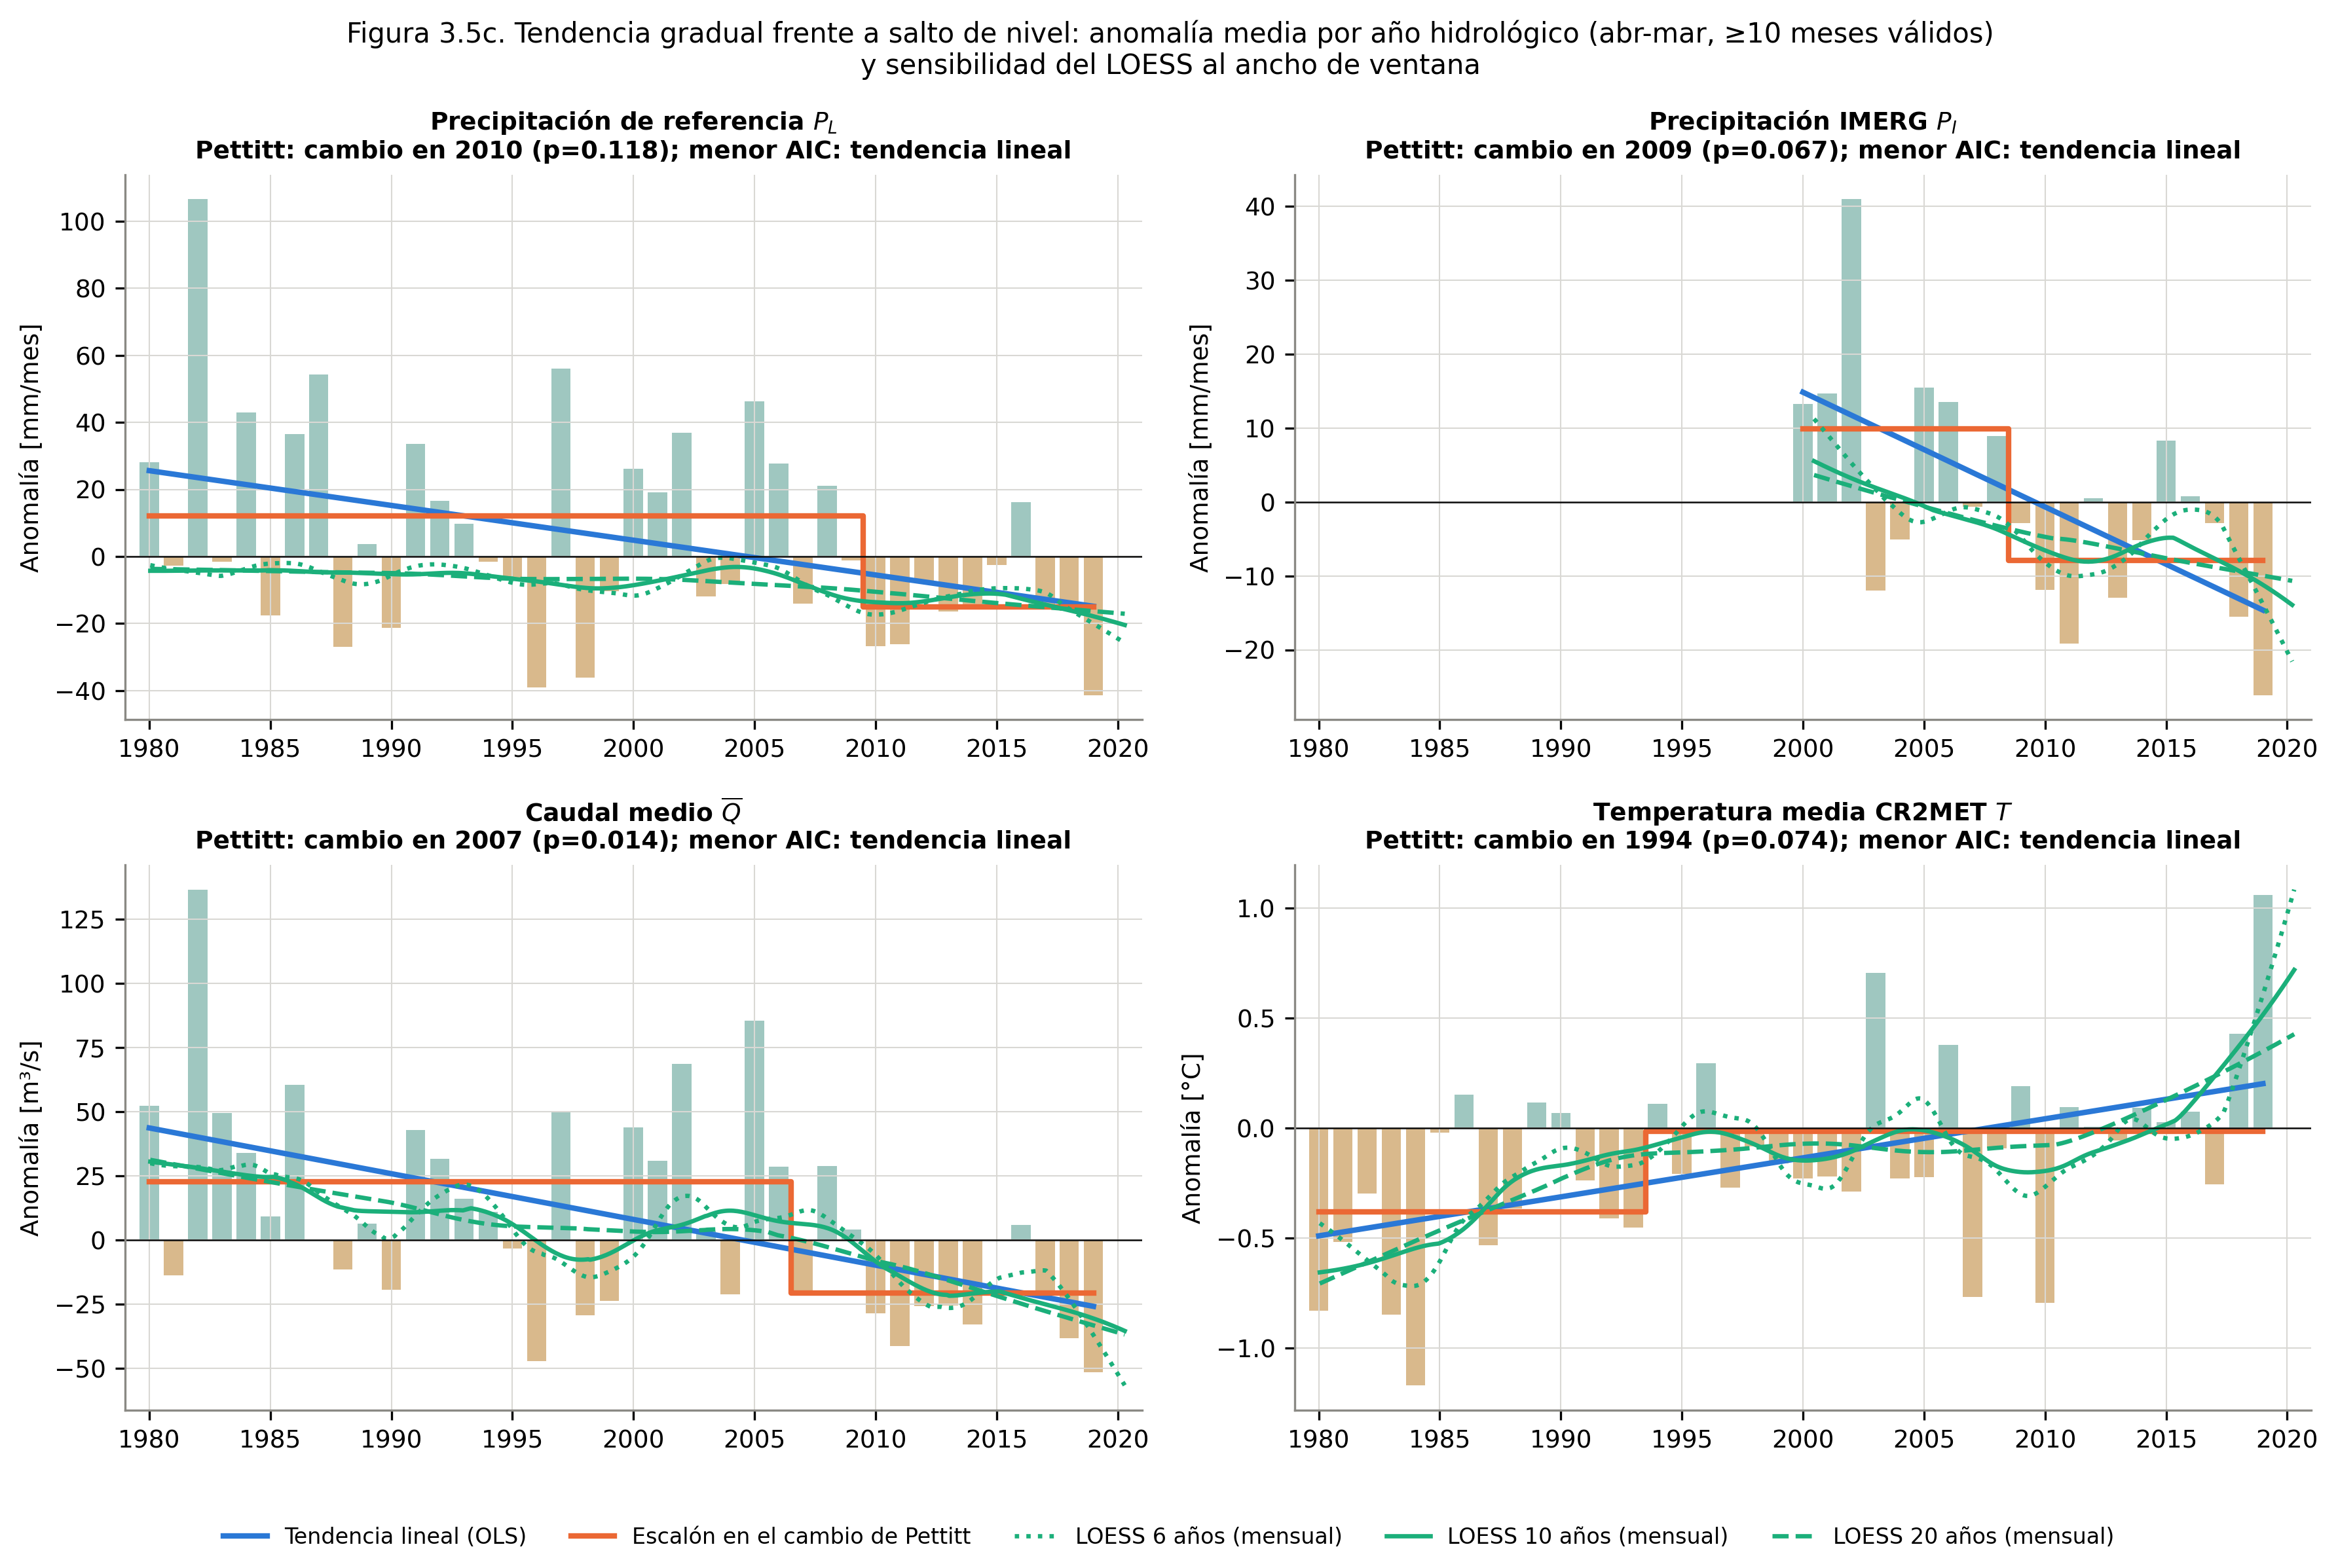
\includegraphics[width=0.9\textwidth]{figura_3_5c_salto_vs_tendencia.png}
\caption{Versión del informe de la diapositiva 02 (figura 3.5c).}
\end{figure}

\paragraph{Cómo se lee la gráfica.} Cada barra es la anomalía media de un año hidrológico (abril a marzo).
La línea azul es una tendencia lineal y la línea escalonada es un cambio de nivel en el año que detecta la
prueba de Pettitt. Si una de las dos líneas ajustara mucho mejor, sabríamos qué tipo de cambio es.

\paragraph{Lo fundamental.} Hay barras positivas y negativas mezcladas hasta $\sim$2009 y casi todas
negativas después. Por eso, \textbf{sin la década de 2010 no hay tendencia significativa}. La tendencia de
40 años la produce, en su mayor parte, la megasequía. Ambos modelos ajustan igual, así que es honesto decir
que no sabemos si es un salto o una tendencia.

\begin{guion}
``¿Es un cambio gradual o un salto? Si cortamos el registro en 2009, la tendencia deja de ser significativa,
tanto en la lluvia como en el caudal. La prueba de Pettitt ubica el cambio en 2007 para el caudal y en 2010
para la lluvia, que es el inicio de la megasequía de Chile central. Un modelo de tendencia lineal y uno de
escalón ajustan prácticamente igual, así que no podemos distinguirlos. Lo que sí es robusto es el signo:
aunque quitemos los años más húmedos, como 1982 o 1997, la caída se mantiene.''
\end{guion}

\begin{cifras}
\begin{itemize}
\item Solo 1980--2009: Q $-9.4$ ($p=0.14$); P$_L$ $-6.4$ ($p=0.15$), ninguna significativa.
\item Pettitt: Q en 2007 ($p=0.014$); P$_L$ en 2010 ($p=0.12$). $\Delta$AIC entre tendencia y escalón $\approx0.2$.
\item El 85--86\,\% de las ventanas de al menos 15 años tienen pendiente negativa.
\end{itemize}
\end{cifras}

\paragraph{Si te preguntan\ldots}
\begin{itemize}
\item \emph{¿Entonces la tendencia es falsa?} No: es real en el periodo observado, pero no es una pendiente
constante que se pueda extrapolar. Describe un periodo húmedo al inicio y uno seco al final.
\item \emph{¿Por qué año hidrológico?} Porque abril--marzo no parte en dos el invierno lluvioso ni el verano de
deshielo; es la convención de la DGA en Chile.
\end{itemize}

% -----------------------------------------------------------------------------
\section{Diapositiva 03 --- ¿A qué se debe? (45 s) --- la más importante}

\paragraph{Cómo se lee la gráfica.} Hay dos series por año hidrológico: la precipitación total (P) y la
escorrentía total (R, el caudal convertido a lámina en mm). Las líneas discontinuas son las medias de
1980--2009 y de 2010--2019. Al estar en las mismas unidades (mm/año) se comparan directamente.

\paragraph{Lo fundamental.} Las dos bajan casi en la misma proporción: P un 39\,\% y R un 42\,\%. Eso responde
la pregunta 3.6.1 (¿el caudal responde de manera consistente con la precipitación?): \textbf{sí}. La
explicación más sustentada es entonces el déficit de lluvia (H1), y no una causa local como un embalse, que
afectaría solo ciertos meses. El pequeño déficit adicional ($-23$~mm/año tras descontar la lluvia del año y la
del año anterior) es compatible con la memoria hidrológica: los almacenamientos de nieve y agua subterránea se
van vaciando durante una sequía de varios años.

\begin{guion}
``¿A qué se debe? Comparamos en las mismas unidades la lluvia y la escorrentía de cada año. Desde 2010, la
lluvia bajó un 39\,\% y la escorrentía un 42\,\%: el río responde en proporción a la lluvia perdida. Por eso
nuestra hipótesis mejor sustentada es el déficit de precipitación invernal de la megasequía, que reduce la
nieve acumulada y con ella el deshielo. Además, aun descontando la lluvia del año y la del anterior, queda un
déficit pequeño, coherente con el agotamiento de almacenamientos que describen Alvarez-Garreton y colegas para
cuencas chilenas con memoria larga. El calentamiento y la regulación del embalse El Yeso son plausibles,
pero con nuestros datos no podemos probarlos. Y una tendencia por sí sola no demuestra una causa, ni siquiera
el cambio climático.''
\end{guion}

\begin{cifras}
\begin{itemize}
\item P: 915 $\rightarrow$ 557~mm/año ($-39$\,\%); R: 822 $\rightarrow$ 475~mm/año ($-42$\,\%); elasticidad $\approx1.1$.
\item $R/P\approx0.9$ sin tendencia significativa. Residuo de R: $+8 \rightarrow -23$~mm/año.
\item Solo 9 años completos después de 2010 (27 antes): es evidencia débil para la memoria hidrológica.
\end{itemize}
\end{cifras}

\paragraph{Las cuatro hipótesis en orden de evidencia} (las mismas de la diapositiva):
\begin{enumerate}
\item \textbf{Fuerte}: déficit de lluvia invernal $\rightarrow$ menos nieve $\rightarrow$ menos caudal todo el año.
\item \textbf{Moderada}: memoria hidrológica (se vacían la nieve remanente y los acuíferos).
\item \textbf{Abierta}: calentamiento (no significativo en 20 años de reanálisis) y regulación o extracciones
(El Yeso existe desde los años sesenta, antes del registro, y la caída es proporcional y ocurre en todos los
meses).
\item \textbf{Cautela}: el registro empieza húmedo (El Niño de 1982 y 1987) y termina seco; además, los
productos de lluvia podrían no ser homogéneos (IMERG cambia de era TRMM a GPM en 2014).
\end{enumerate}

\paragraph{Si te preguntan\ldots}
\begin{itemize}
\item \emph{¿Por qué $R/P\approx0.9$ es tan alto?} Es sospechoso para una cuenca semiárida. Probablemente
P$_L$ subestima la precipitación de alta montaña, o hay aporte glaciar. Por eso usamos los cambios
\emph{relativos} y no cerramos un balance.
\item \emph{¿Y los rezagos?} El caudal tiene una persistencia mensual de 0.78--0.81 y el Rol B encontró un
máximo de asociación cerca de 6--7 meses; un déficit de lluvia afecta varios meses de caudal.
\item \emph{¿Y IMERG?} Coincide en el signo, pero cae menos que P$_L$ en el periodo común ($-15.5$ frente a
$-24.3$): las fuentes discrepan en la magnitud.
\end{itemize}

% -----------------------------------------------------------------------------
\section{Diapositiva 04 --- ¿En qué escalas varía? (40 s)}

\begin{figure}[H]
\centering
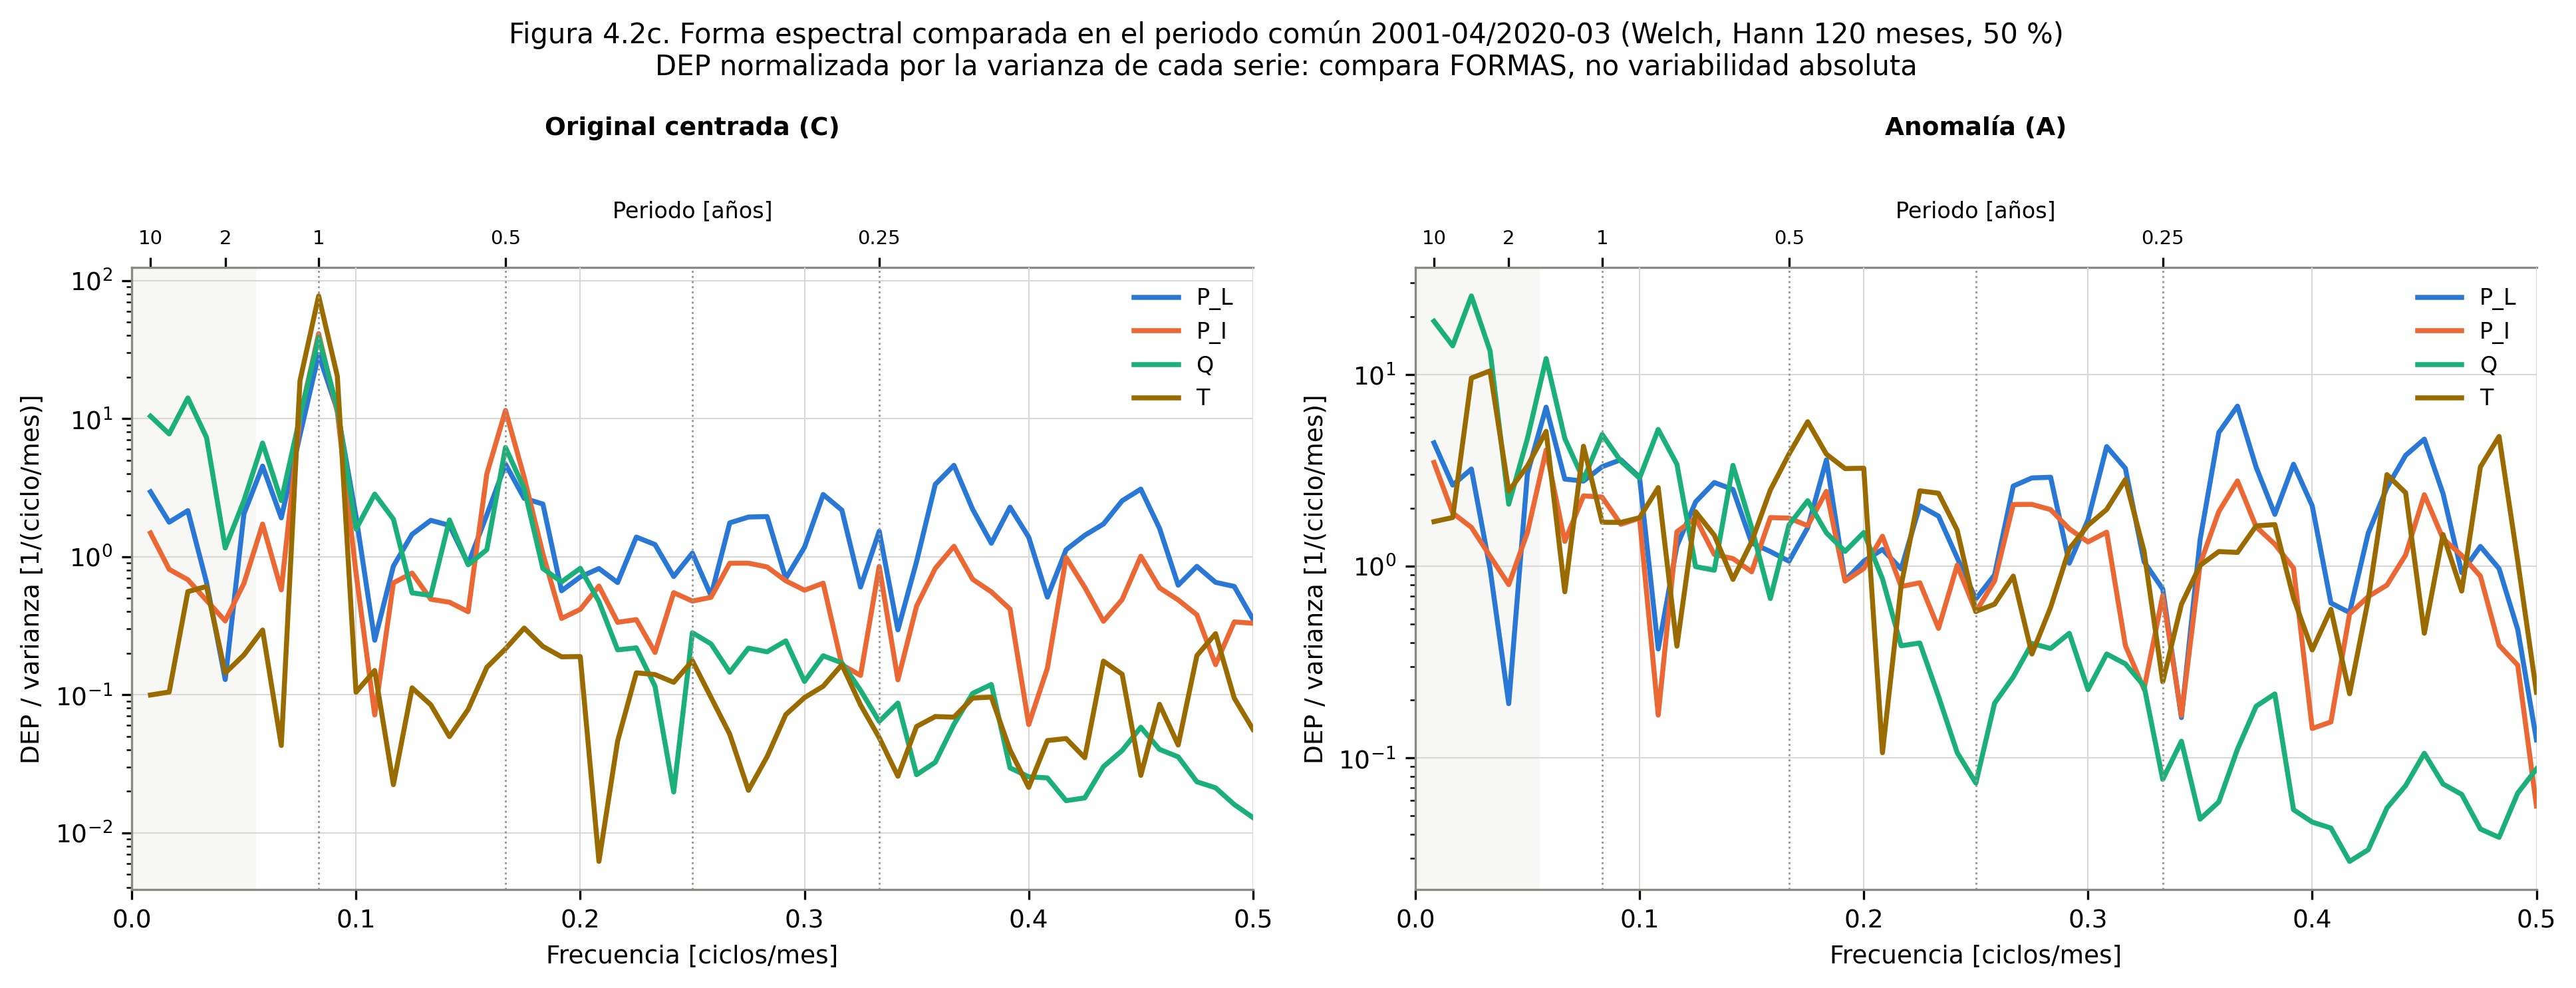
\includegraphics[width=0.95\textwidth]{figura_4_2c_espectros_normalizados.png}
\caption{Versión del informe (figura 4.2c). La diapositiva muestra P$_L$ y Q en 1980--2020 con su ruido rojo
AR(1) de referencia.}
\end{figure}

\paragraph{Cómo se lee la gráfica.} El eje x es la frecuencia en ciclos por mes: a la izquierda están las
variaciones lentas (de varios años) y a la derecha las rápidas (de 2--3 meses). El eje y indica cuánta
varianza hay en cada frecuencia, normalizada para comparar formas. La línea discontinua es lo que daría un
ruido rojo AR(1) con la misma persistencia: un pico real debería sobresalir claramente de ella.

\paragraph{Lo fundamental.} El espectro de las anomalías de lluvia es casi plano (ruido blanco: la lluvia de
un mes casi no recuerda la del anterior). El del caudal cae fuertemente hacia la derecha (ruido rojo): el río
apaga lo rápido y conserva lo lento. Es la firma espectral del almacenamiento y la misma física de las
diapositivas 01 y 03, vista desde otro ángulo.

\begin{guion}
``En el análisis de Fourier, el único pico robusto es el ciclo anual, que explica el 93\,\% de la varianza de
la temperatura, cerca de la mitad en caudal e IMERG y un tercio en la lluvia de referencia. El pico de seis
meses es solo un armónico, porque el ciclo no es sinusoidal. Al quitar el ciclo anual aparece lo
interesante: las anomalías de lluvia son casi ruido blanco, pero las de caudal son ruido rojo, con el 60\,\%
de su varianza en escalas de más de año y medio. La cuenca funciona como un filtro: la nieve, los glaciares
y el agua subterránea integran la lluvia. Ningún pico interanual supera el umbral global de ruido rojo, así
que no afirmamos ningún ciclo, ni siquiera ENSO, que se evalúa en el punto 5.''
\end{guion}

\begin{cifras}
\begin{itemize}
\item Fracción anual en la serie original: T 93\,\%, P$_I$ 55\,\%, Q 46\,\%, P$_L$ 32\,\%.
\item Anomalías: persistencia r$_1$ de 0.15 (P$_L$) frente a 0.81 (Q); varianza interanual 15\,\% frente a 60\,\%.
\item Periodo interanual dominante inestable: 2.7 años (Hann), 20 (boxcar), 1.7 (Welch).
\end{itemize}
\end{cifras}

\paragraph{Si te preguntan\ldots}
\begin{itemize}
\item \emph{¿Cómo trataron los vacíos?} Solo el caudal tiene vacíos (14 meses). Interpolamos la anomalía, no
pusimos ceros ni concatenamos meses. Comprobamos que no importa: el tramo continuo 1990--2014 y Lomb--Scargle
sin relleno dan la misma fracción interanual.
\item \emph{¿Por qué la ventana Hann?} Reduce la fuga espectral del pico anual hacia las frecuencias vecinas, a
costa de algo de resolución. Usamos además años completos (N = 480) para que el ciclo anual cupiera un número
entero de veces.
\item \emph{¿Qué es el umbral global?} Probamos unas 240 frecuencias: al 5\,\%, unas 12 superarían un umbral
puntual solo por azar. El umbral global corrige esa búsqueda y lo estimamos con 1000 simulaciones AR(1).
\item \emph{¿El espectro muestra el desfase lluvia--caudal?} No. Un espectro de potencia no contiene la fase;
el desfase de 6--7 meses viene de la climatología y de los rezagos.
\end{itemize}

% -----------------------------------------------------------------------------
\section{Diapositiva 05 --- Síntesis (20 s)}

\begin{guion}
``En síntesis: el caudal del Maipo disminuyó en todos los meses, sobre todo después de 2010. Se explica
principalmente por la menor lluvia invernal, transmitida por el almacenamiento nival, que también hace que el
río tenga memoria de varios años. La hipótesis nivo-pluvial del punto 1 se mantiene, pero lo que vemos es una
megasequía en un registro corto, no un ciclo ni una tendencia que se pueda extrapolar.''
\end{guion}

% -----------------------------------------------------------------------------
\section{Lo que NO debes decir}

\begin{itemize}
\item ``La tendencia demuestra el cambio climático.'' Una tendencia aislada no atribuye una causa (3.6.4).
\item ``La temperatura aumentó significativamente.'' No lo hizo: $p=0.27$, 20 años de reanálisis.
\item ``Hay un ciclo de 2.7 años'' o ``hay un ciclo de ENSO''. Ningún pico interanual es robusto ni significativo.
\item ``El caudal va a seguir bajando 18~m$^3$/s por década.'' No se extrapola: el cambio parece un salto.
\item ``El espectro muestra que el caudal se retrasa 6 meses.'' El espectro de potencia no tiene fase.
\item ``La lluvia bajó un 10\,\%.'' La pendiente es de mm/mes \emph{por década} en el acumulado mensual, no del total anual.
\end{itemize}

\section{Decisiones de método en una línea (para la defensa)}

\begin{table}[H]
\centering\small
\begin{tabularx}{\textwidth}{l X}
\toprule
Decisión & Justificación \\
\midrule
Referencia 2000-06 a 2020-03 & La misma de los roles A y B y la única con las 4 variables. Contra: es un periodo seco e infla $z$ antes de 2000. \\
OLS + HAC & Residuos autocorrelacionados y heterocedásticos. \\
Efectos de mes en X & Sin ellos, T daba $+0.66$ en lugar de $+0.28$ por empezar en invierno y terminar en verano. \\
Kendall estacional + bootstrap & Serie con ciclo anual; los bloques de 3 años conservan la dependencia. \\
Hamed--Rao & Corrige Mann--Kendall por persistencia (factor 6.4 en Q). \\
Sen estacional $\neq$ OLS en P$_L$ & Sen pondera igual los meses secos de verano, que no cambian; la señal es invernal. \\
LOESS & Muestra la forma no lineal; es exploratorio, sin inferencia. \\
Pettitt + AIC & Para distinguir un salto de una tendencia (no se pudo). \\
FDR (Benjamini--Hochberg) & Familias de 48 pruebas mensuales y 12 globales. \\
Hann, Welch y AR(1) por Monte Carlo & Controlar la fuga, la varianza y la búsqueda entre frecuencias. \\
\bottomrule
\end{tabularx}
\end{table}

\end{document}
